\documentclass[a4paper]{article}

%% Language and font encodings
\usepackage[english]{babel}
\usepackage[utf8x]{inputenc}
\usepackage[T1]{fontenc}

%% Sets page size and margins
\usepackage[a4paper,top=3cm,bottom=2cm,left=3cm,right=3cm,marginparwidth=1.75cm]{geometry}

%% Useful packages
\usepackage{amsmath}
\usepackage{graphicx}
\usepackage[colorinlistoftodos]{todonotes}
\usepackage[colorlinks=true, allcolors=blue]{hyperref}

\usepackage{fancyvrb}
\usepackage{alltt}

\title{Actividad 4}
\author{Isaac Neri Gómez Sarmiento}
\date {25 de Febrero del 2018}

\begin{document}
\maketitle


\section{Introducción}

El objetivo de esta actividad es aprender y utilizar los comandos del sistema operativo Unix para la manipulación de archivos y datos. En este caso se descargó la información meteorológica de todo uño (2017) del área esudiada en la práctica pasada, en este caso Brindisi, Italia.

En esta práctica se habla acerca de términos como shells, scripts o Bash. Es importante aclarar estos términos antes de poder avanzar.

Un \textbf{shell} es una interfaz o lugar donde la computadora y el usuario interactuan, tal como su nombre lo indica es el caparazón o capa exterior con el cual estamos "en comunicación" con el sistema operativo que controla y administra los recurso de hardware y software. 

Un \textbf{script} es un programa corto el cual contiene líneas de código para ser ejectudados por un lenguaje de interpretación. Los scripts creados en esta actividad tienen la terminación .sh. Todo script debe contener en el inicio el texto \textbf{ \#!/bin/bash }.

El \textbf{Bash} (\textbf{B}ourne-\textbf{a}gain \textbf{sh}ell) es simplemene un procesador de comandos el cual los lee y los ejecuta. El utilizado en clase usa un \textit{shell prompt}, es decir un caracter "\$" que indica que la computadora está en la espera de recibir una entrada. 



\section{Actividades realizadas}

\begin{enumerate}


\item Se descargó un script llamado "script1" el cual contiene una serie de comandos para automatizar la descarga de información meteorológica de la Universidad de Wyoming de una estación a escoger.

\item Dentro del código se introdujo el número de la estación 16320, que en este caso el que corresponde a Brindisi, Italia.

\begin{verbatim}
#!/bin/bash
STATION=16320
\end{verbatim}

\item Se editó el rango de años de los datos deseados a 2017. 

\begin{verbatim}
LISTYs="2017"
\end{verbatim}

\item Así mismo, se hizo una clasificación de los meses por el número de días.


\begin{verbatim}
LISTM31="01:03:05:07:08:10:12"
LISTM30="04:06:09:11"
LISTM28="02"
\end{verbatim}

\item Se hizo uso de 3 FOR loop para bajar los datos en cada clasificación de los meses; de 28 días, de 30 días y de 31 días. El comando utilizado para abrir la página web desde la terminal fue: \begin{verbatim} /usr/bin/wget \end{verbatim}  seguido por la URL entre comillas. 

\newpage

Entre cada descarga y otra se utilizó el comando \begin{verbatim} /bin/sleep 10 \end{verbatim}  para que se esperara 10 segundos entre una descarga y otra. 


\begin{verbatim}
for j in $LISTYs ; do

### Meses 31 dias
for i in $LISTM31 ; do
	/usr/bin/wget "http://weather.uwyo.edu/cgi-bin/sounding?region=naconf&TYPE=TEXT%3ALIST&YEAR=$j&MONTH=$i&FROM=0100&TO=3112&STNM=$STATION"
        /bin/sleep 10
done
### Meses 30 dias
for i in $LISTM30 ; do
	/usr/bin/wget "http://weather.uwyo.edu/cgi-bin/sounding?region=naconf&TYPE=TEXT%3ALIST&YEAR=$j&MONTH=$i&FROM=0100&TO=3012&STNM=$STATION"
        /bin/sleep 10
done
### Feb. 28 dias
for i in $LISTM28 ; do
	/usr/bin/wget "http://weather.uwyo.edu/cgi-bin/sounding?region=naconf&TYPE=TEXT%3ALIST&YEAR=$j&MONTH=$i&FROM=0100&TO=2812&STNM=$STATION"
        /bin/sleep 10
done
done
\end{verbatim}

\item Se utilizaron comandos como: \textit{less, cat, grep, diff}, entre otros para la visualización y manipulación de los datos.
\end{enumerate}

\section{Comandos aprendidos}
\subsection{cat}
Este tiene 3 funciones principales:
\begin{itemize}

\item Desplegar archivos de texto
\item Crear nuevos archivos de texto
\item Combinar copias de archivos de textos (concatenación)

\end{itemize} 


Para mostrar en la terminal un script llamado "ejemplo1.sh" se escribe en la terminal:
\begin{verbatim}
cat ejemplo1.sh
\end{verbatim}

Para copiar datos de un archivo a uno nuevo:

\begin{verbatim}
cat ejemplo1.sh >ejemplo2.sh
\end{verbatim}

Para crear un archivo de texto nuevo con la información escrita en la terminal, se escribe:

\begin{verbatim}
cat> Saludo
Hola mundo
\end{verbatim}

Para indicarle a la terminal que ya terminamos, presionamos Ctrl+d.De esta manera se creó un archivo llamado Saludo que contiene "Hola mundo". 


Para concatenar o juntar una serie de archivos en uno solo se puede escribir en la terminal:

\begin{verbatim}
cat ejemplo1 ejemplo2 ejemplo3 > ejemplo4 
\end{verbatim}

\subsection{chmod}

Este se utiliza para dar permisos de lectura, escritura o ejecución al usuario, a grupos u a otros. 
Para ver los permisos que tienen los scripts se utiliza el comando "ls-l", por ejemplo:
\begin{verbatim}
ls -l ex1
\end{verbatim}

Lo cual imprime en pantalla:
\begin{verbatim}
-rw-r--r-- 1 nikoneri users 5 feb 21 11:37 ex1
\end{verbatim}

El primer caracter "-" representa el tipo de archivo, "-" para un arhivo regular, "d" para un directorio y "I" para un link simbólico.

Los 3 caracteres que siguen “rw-” representan los permisos del usuario, Se le permite leer “r”, se le permite escribir “w”, no se le permite ejecutar “-”. Si se le permitiera estuviera un “x” en lugar de un “-”.

Los 3 caracteres que siguen “r--” representan los permisos para grupo. Se le permite al grupo leer “r”, no se le permite escribir ni ejecutar “--”

Los 3 últimos 3 caracteres “r--” representan los permisos para otros. Solamente se le permite leer “r”, pero no escribir ni ejecutar “--”.

Para poder asignar permisos, se asigna números  a las acciones de read, write, execute y ningún permiso.

\begin{itemize}
\item Read: 4
\item Write: 2
\item Execute: 1
\item Ningún permiso: 0
\end{itemize}

Por ejemplo, si escribimos en la terminal:

\begin{verbatim}
chmod 745 ex1
\end{verbatim}

El primer digito 4+2+1=”7” permite al usuario Leer, Escribir, Ejecutar el archivo "ex1"
El segundo digito “4” solamente permite al grupo Leer el archivo "ex1".
El tercer digito  4+1=”5” permite a otros Leer y ejecutar el archivo "ex1"

\subsection{echo}

Este comando imprime texto en pantalla o en un documento. También muestra el valor de variables creadas.
 \begin{verbatim}
echo Hola mundo>Saludo
 
cat Saludo
 \end{verbatim}
Al usar el comando cat para ver el contenido del archivo Saludo, aparece:
\begin{verbatim} 
Hola mundo
\end{verbatim}
Para guardar texto o numeros en variables y poder mostrarlas también se utiliza el echo:

\begin{verbatim}
X=3.1415

echo El valor aproximado de pi es $X
\end{verbatim}
por lo que se imprime en pantalla:

\begin{verbatim}
El valor aproximado de pi es 3.1415
\end{verbatim}

\subsection{grep}

Se utiliza para buscar determinado texto contenido en un archivo, por ejemplo:

\begin{verbatim}
grep "Caldo" Menu

Caldo de res
Caldo de camaron
Caldo de pollo
\end{verbatim}

\subsection{less}
Este permite ver el contendio de un archivo, pantalla por pantalla al presional la barra de espacio y para moverse hacia atrás presionando “b”. Para salir de “less” solo se debe presionar “q”. Ejemplo:

\begin{verbatim}
cat file1 | less 
\end{verbatim}

Este comando es muy útil a la hora ed desplegar una inmensa cantidad de datos en la terminal, ya que se puede visualizar pantalla por pantalla la información.

\subsection{wc}

El comando wc es un acrónimo de "wordcount" y éste despliga información acerca de un achivo, tal y como: número de lineas, número de palabras y número de caracteres. Por ejemplo:

\begin{verbatim}
wc ex4
6 12 60 ex4
\end{verbatim}
Lo anterior nos indica que el archivo ex4 contiene 6 lineas, 12 palabras y 60 caracteres.

\section{Resúmen \textit{Shell Script Tutorial}}

\subsection{Introduction}

Los puntos más importantes que se pueden rescatar son:

\begin{itemize}

\item El creador del Bourne shell fue Steve Bourne, asociado a los laboratorios Bell Labs. 
\item Las entradas en las líneas de comandos estarán precedidas por el símbolo de dolar "\$". 
\item Cualquier script comienza por \textbf{ \#!/bin/bash } en la primera línea.
\item Para activar el permiso de modificación y lectura a un archivo, se escribe:
\end{itemize}
\begin{verbatim}
$ chmod a+rx ejemplo1.sh
./ejemplo1.sh
\end{verbatim}

\subsection{Philosophy}
Esta sección no tiene mucha información relevante, no obstante los puntos que se pueden rescatar en cuanto a la creación de buenos scripts son:
\begin{itemize}
\item Mantener un diseño claro y legible
\item Evitar comandos innecesarios
\item Indentar estructuras de control como if/then/else para un mejor orden
\end{itemize}


\subsection{A first script}

En esta sección se da un ejemplo de cómo hacer un script básico. Haremos uno similar.

\begin{verbatim}
#!/bin/bash
  echo Salut tout le monde
\end{verbatim}

Para activar los permisos de ejecución para el usuario se escribe en la terminal:

\begin{verbatim}
$ chmod 755 Saludo.sh
$ ./Saludo.sh
Salut tout le monde 

\end{verbatim}

\subsection{Variables-Part I}

Las variables son nombres simbólicos a través de los cuales se pueden asignar valores, leerlos o manipular sus contenidos. 

Para la asignación de variables se debe colocar el signo "=" sin espacios entre el nombre de la variable y el valor. 



\begin{verbatim}

VAR=value #Funciona

VAR = value #No funciona
\end{verbatim}

Un ejemplo de asignación a variables es el sig:

\begin{verbatim}
#!/bin/sh
echo Tu t'appelle comment?
read nom
echo "Salut $nom - J'espère que tu vas bien."
\end{verbatim}

La salida en la terminal es:

\begin{verbatim}
$ chmod 755 Saludo2.sh
$ ./Saludo2.sh
Tu t'appelle comment?
Isaac #Aqui se introdujo el nombre
Salut Isaac - J'espère que tu vas bien.
\end{verbatim}

Las variables en el Bourne shell no tienen que ser declarados tal y como en Fortran se hace. Pero si se trata de leer una variable no asignada el resultado es un espacio en blanco, por ejemplo.

\begin{verbatim}
#!/bin/sh
echo "Saludo: $Saludo"
Saludo="Bonjour"
echo "Saludo: $Saludo"
\end{verbatim}

Después de correr el script
\begin{verbatim}
$ chmod 755 Saludo3.sh
$ ./Saludo3.sh
Saludo:
Saludo: Bonjour
\end{verbatim}


\subsection{Wildcards}
Los wildcards se representan por los siguientes caracteres:

\begin{itemize}
\item * - representa cero o más caracteres
\item ? - representa un caracter
\item \*[ ] - representa un rango de caracteres
\end{itemize}

Si queremos por ejemplo enlistar los archivos que comienzen por c
 
\begin{verbatim}
$ ls C*
carta.txt coche.txt
\end{verbatim}

En realidad el sistema identifica todos los archivos que contengan c al principio e intercambia el ls c* por un ls carta.txt coche.txt y luego ejectua el comando ls. 

Este wildcard fue utilizado en el paso 13 de la actividad, al usar:

\begin{verbatim}
sounding* > sondeos.txt
\end{verbatim}

Lo que hizo en realidad fue tomar una copia de cada archivo que comenzara por sounding (que en nuestro caso eran 12 archivos de datos, uno por cada mes) y las concatenó en un solo archivo.

\subsection{Escape Characters}
Los escape characters son caracteres especiales tales como:

\begin{itemize}
\item  \textbackslash
\item  \$
\item  "
\end{itemize}

El " es especial para preservar los espacios. 

\begin{verbatim} 
$ echo Hola      Mundo
Hola Mundo
$echo "Hola      Mundo"
Hola      Mundo
\end{verbatim}

El símbolo de pesos usado antes de una variable, la marca para que muestre el valor que se le asignó.

\begin{verbatim}
$ X=20
$ echo "Tengo $X años de edad"
Tengo 20 años de edad
\end{verbatim}


El backslash es usado para desenmarcar algunos caracteres. Por ejemplo si quiero imprimir en pantalla  una frase con comillas.

\begin{verbatim}
$ echo "Calcaneo dijo: \"FORTRANlezcase con una buena dosis de análisis numérico.\" "

Calcaneo dijo: "FORTRANlezcase con una buena dosis de análisis numérico."
\end{verbatim}

\subsection{Loops}

Los loops o ciclos ayudan a repetir un comando varias veces. En el caso de \textbf{for} loops, estos iteran un conjunto de datos hasta que la lista se haya acabado. Por ejemplo:


\begin{verbatim}
#!/bin/sh
echo "Cuenta regresiva"
for i in 5 4 3 2 1
do 
    echo "$i"
done
echo ¡Despegue!
\end{verbatim}

Por lo que el resultado es:


\begin{verbatim}
$ chmod 755 cuenta_regresiva.sh
$ ./cuenta_regresiva.sh
Cuenta regresiva
5
4
3
2
1
¡Despegue!
\end{verbatim}

El loop \textbf{while} itera una serie de comandos hasta que se cumple una condición específica. Por ejemplo:

\begin{verbatim}
#!/bin/sh
Salutations=Bonjour
while ["Salutations" != "Au revoir" ]
do
	echo "Ecrivez quelque chose (Au revoir pour quitter)"
    read Salutations
    echo "Vous avez écrit: $Salutations"
done
\end{verbatim}

Por lo que la salida del código anterior es:

\begin{verbatim}

$ chmod 755 Saludo4.sh
$ ./Saludo4.sh
Ecrivez quelquechose (Au revoir pour quitter) 
Hola #Este es la entrada que se escribió en la terminal
Vous avez écrit: Hola
Ecrivez quelquechose (Au revoir pour quitter) #Se vuelve a repetir hasta que escribamos Au revoir.
Au revoir
$

\end{verbatim}

\subsection{Test}

Este comando normalmente se utiliza para hacer pruebas, tal como su nombre lo indica cuyos valores que regresa es un 0 si es TRUE la comparación o 1 si es FALSE la comparación de las expresiones.Por ejemplo:

\begin{verbatim}
#!/bin/sh
x=10
y=15
test $x -eq  $y && echo "$x si es igual a $y " || echo "$x no es igual a $y"
\end{verbatim}

Por lo que la salida es:

\begin{verbatim}
$ chmod 755 test1.sh
$ ./test1.sh
10 no es igual a 15
\end{verbatim}

Otro ejemplo usando strings:
\begin{verbatim}
#!/bin/sh
x="Caldo de pollo"
y="Caldo de res"
[ "$x" = "$y" ]; echo $? 
\end{verbatim}
Imprimiendo en pantalla el número 1, lo cual significa que son diferentes. En el caso que hayan sido iguales, hubiera impreso el número 0.


\subsection{Case}
El case es una estructura de control que permite escoger entre una variedad de casos donde cada uno tiene cierta función. Por ejemplo:

\begin{verbatim}
#!/bin/sh
echo "Dime con qué programas y te diré quien eres"

	read entrada
    case $entrada in
    Fortran)
    	echo "Eres físico"
        ;;
	Maple)
    	echo "Eres matemático
        ;;
    *)
    	echo "Ni idea quien eres"
        ;;
    esac #Se debe poner esac para terminar un case	
\end{verbatim}

La salida en la terminal sería:

\begin{verbatim}
$ chmod 755 encuesta_prog.sh
$ ./encuesta_prog.sh
Dime con qué programas y te diré quien eres
Fortran #Aquí escribí la entrada
Eres físico
\end{verbatim}

\subsection{Variables-Part II}
Existen ciertas variables predeterminadas que en algunos casos no se le pueden asignar valores. 
En el texto leído se refieren a ellas como parámetros. Ejemplos de las variables predeterminadas mencionadas son:

\begin{verbatim}
$#, $1, $2, ..., $9
\end{verbatim}

A continuación se da un ejemplo en donde se muestra primero un script que hace uso de tales variables, depués se ejecuta el script sin valores asignados a las variables y finalmente se ejecuta con valores asignados a las variables.

\begin{verbatim}
#!/bin/sh
echo "Se han utilizado $# parametros"
echo "El nombre de este archivo es: $0"
echo "El primer parámetro  es $1"
echo "El segundo parámetro es $2"
echo "Todos los parámetros son $@"
\end{verbatim}

\begin{verbatim}
$ chmod 755 variables
$./variables.sh
Se han utilizado 0 parametros
El nombre de este arhivo es /Computacional/Actividad4/variables.sh
El primer parametro es 
El segundo parametro es  
Todos los parámetros son
$
$./variables.sh Caldo con pollo
Se han utilizado 3 parametros
El nombre de este archivo es ./var3.sh
El primer parametro es Caldo
El segundo parametro es con
Todos los parámetros son Caldo con pollo
\end{verbatim}

Otra variable interesante es ?\#, la cual almacena el valor del último comando ejecutado. Un ejemplo que puse anteriormente contiene esta variable:

\begin{verbatim}
$ x="Caldo de pollo"
$ y="Caldo de res"
$ [ "$x" = "$y" ]; echo $? 

\end{verbatim}
En este caso el valor que almacena \$? es un 1, ya que x es diferente de y. 

La variable \textbf{IFS} (Internal Field Separator) es un separador que sirve a la hora de enlistar una serie de archivos, pueden ser con espacios, coma, dos puntos, etc. Esto depende de qué caracter se le asigne, por ejemplo:

\begin{verbatim}
#!/bin/sh
old_IFS="$IFS"
IFS=,
echo "Introduzca 3 datos separados por coma"
read a b c
IFS=$old_IFS
echo "a es $a, b es $b, c es $z"
\end{verbatim}

La variable \textbf{\$\$} se utiliza para crear archivos temporales tales como 
\begin{verbatim}
/tmp/ejemplo.$$
\end{verbatim}

\subsection{Variables Part 3}
Las llaves usadas a la hora de imprimir una variable son convenientes para evitar confusiones, por ejemplo:

\begin{verbatim}
$ var=cere
$ echo $varbro #$varbro no está definido

$ echo ${var}bro 
cerebro
\end{verbatim}

El uso de  \textbf{`whoami`} indica el nombre del usuario de la sesión.

Para especificar un valor default cuando a una variable no se le ha asignado algún valor o expresión, se hace uso del \textbf{:-}, por ejemplo:

\begin{verbatim}
echo -en "Cómo te llamas [ `whoami` ] "
read myname
echo "Mi nombre es : ${myname:-`whoami`}"
\end{verbatim}

El comando \textbf{-en} después del echo funciona para no añadir un salto de línea a la hora de realizar la lectura, sino en la misma línea. 
En el sig. ejemplo no se escribe una entrada, por lo que la salida es el usuario de la sesión.

\begin{verbatim}
$ chmod 755 whoamI.sh
$ ./whoamI.sh
Cómo te llamas [nikoneri]
Tu nombre es: nikoneri
\end{verbatim}

Y en el caso en el que se haya introducido un nombre.
\begin{verbatim}
$ chmod 755 whoamI.sh
$ ./whoamI.sh
Cómo te llamas [nikoneri] Isaac
Tu nombre es: Isaac
\end{verbatim}

\subsection{External Programs}

El comando externo backtick (`) es usado para  poder guardar la salida externa de cualquier comando en una variable.Un ejemplo muy simple es el siguiente:

\begin{verbatim}
$ Var=`echo La Real Academia de`
$ echo $Var Probabilidad
\end{verbatim}

Donde la salida es:
\begin{verbatim}
La Real Academia de Probabilidad
\end{verbatim}

\subsection{Functions}
Para hacer una función, se debe seguir la siguiente estructura:

\begin{verbatim}
nombre_de_la_funcion () { 
  lista de comandos
}
\end{verbatim}

Un ejemplo de una función simple:

\begin{verbatim}
#!/bin/sh
Saludo() {
echo "Hola mundo"
}
\end{verbatim}
Al utilizarla, obtenemos lo siguiente: 
\begin{verbatim}
$ chmod 755 funcion_Saludo.sh
$ ./funcion_Saludo.sh
$ Saludo
Hola mundo
\end{verbatim}


Normalmente las variables son globales, pero en las funciones se pueden usar variables locales las cuales solo se puden usar solo dentro de ella y no por fuera. Por ejemplo:

\begin{verbatim}
#!/bin/sh
Saludo () {
    local var="Hola mundo"
    echo $var
}

\end{verbatim}

Al imprimir la variable var fuera de la función, solo aparece un espacio en blanco. En cambio si hace una llamada a la función "Saludo", se imprime "Hola mundo".

\begin{verbatim}
$ chmod 755 funcion_localvar.sh
$ ./funcion_localvar.sh
$ echo $var
          #Espacio en blanco
$ Saludo
Hola mundo
\end{verbatim}



\subsection{Hints and Tips}
Algunos comandos que se usan en este capítulo son:

\begin{itemize}
\item \textbf{cut}

El uso más sencillo con el que se utiliza este comando es el de seleccionar una columna de caracteres.Por ejemplo, en el siguiente texto seleccionaremos la 3era columna.

\begin{verbatim}
$ cat menu.txt
Pizza
Quesadillas de huitlacoche
Hamburguesa
\end{verbatim}

De esta manera obtenemos:

\begin{verbatim}
$ cut -c3 menu.txt
z
e
m
\end{verbatim}


\item \textbf{grep}

Este comando ya se había descrito en páginas anteriores. Se utiliza para buscar determinado texto contenido en un archivo, por ejemplo:

\begin{verbatim}
$ grep "Caldo" menu2.txt
Caldo de res
Caldo de camaron
Caldo de pollo
\end{verbatim}

\item \textbf{sed}

Este comando se usa para modificar cada linea de un archivo, reemplazando partes de la linea. Por ejemplo, tenemos la siguiente lista de precios de un menu.

\begin{verbatim}
$ cat menu2_precios.txt
1, Caldo de Res, $60
2, Caldo de Pollo, $50
3, Caldo de Camarón, $100
\end{verbatim}

Si quisieramos cambiar el precio del caldo de pollo a \$60, se utiliza el comando sed:

\begin{verbatim}
$ sed 's/50/60/' menu2_precios.txt > menu2_nuevos_precios.txt
\end{verbatim}

El precio del caldo de pollo ya se ha modificado:

\begin{verbatim}
$ cat menu2_nuevos_precios.txt
1, Caldo de Res, $60
2, Caldo de Pollo, $60
3, Caldo de Camarón, $100
\end{verbatim}


\item \textbf{awk}

El uso más básico de este comando es para copiar una columna de un archivo de texto y ponerlos en otro.Por ejemplo, si solamente quisieramos la lista de precios del archivo menu2\_nuevos\_precios.txt.

\begin{verbatim}
$ cat menu2_nuevos_precios.txt
1, Caldo de Res, $60
2, Caldo de Pollo, $60
3, Caldo de Camarón, $100
\end{verbatim}

El comando a escribir para extraer los precios, considerando la separación del texto por espacios:
\begin{verbatim}
$ awk '{ print $5 }' menu2_nuevos_precios.txt > precios.txt
\end{verbatim}

Por lo que la salida sería:

\begin{verbatim}
$60
$60
$100
\end{verbatim}

Considerando que la separación del texto está dada por comas, entonces el comando sería como sigue:

\begin{verbatim}
$ awk -F, '{ print $3 }' menu2.txt > precios.txt
\end{verbatim}
\end{itemize}


\subsection{Quick reference}
En esta sección se da una tabla de los comandos cuya función no siempre se puede inferir de su nombre. Estos ejemplos incluyen \textit{process management}, \textit{shell scripts arguments} y \textit{shell script test conditions}.

\begin{figure}[ht!]
\centering
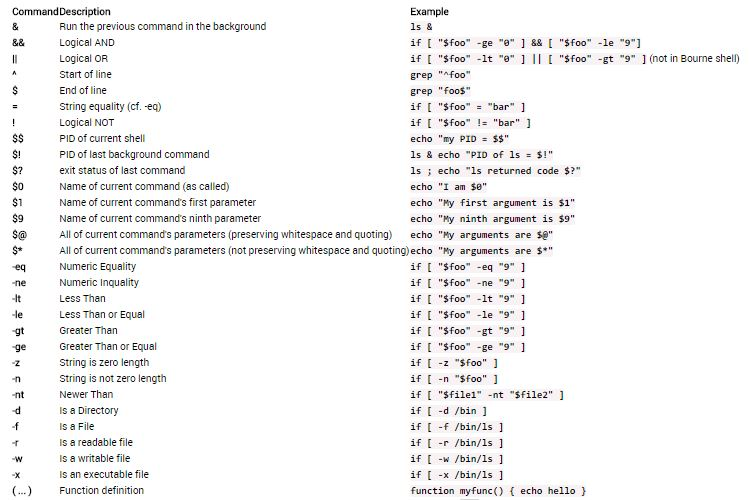
\includegraphics[width=1\textwidth]{Quick_reference.JPG}
\caption{\label{fig:}Referencias de algunos comandos y códigos}
\end{figure}

\newpage

\subsection{Interactive Shell}

El \textit{bash shell} tiene algunas herrramientas útiles para la búsqueda del historial de comandos utilizados anteriormente. Por ejemplo, las flechas hacia arriba y hacia abajo permiten ver los comandos previos. Otro comando es Ctrl+r, el cual hace una búsqueda hacia atrás, coincidiendo cualquier parte de la linea de comandos. Si presionamos ESC, el comando seleccionado será pegado el shell actual para poder editarse.


\section{Apéndice}


\begin{enumerate}

\item ¿Qué fue lo que más te llamó la atención en esta actividad?

La gran variedad de comandos con los que cuenta Linux, los cuales pueden ahorrarnos varios clics. Mas que nada la concatenación de varios archivos en uno solo y la descarga multiple.

\item ¿Qué consideras que aprendiste?

Cómo descargar multiples datos, concatenarlos en un solo archivo, seleccionar ciertas columnas para ponerlas en otro archivo. Creación de funciones y utilización de las estructuras case y loops.

\item ¿Cuáles fueron las cosas que más se te dificultaron?

Mas que nada fueron los ejemplos y las explicaciones que mostraba la página de \textit{Shell Scripting Tutorial} ya que para ejemplificar algunos comandos, a mi parecer a veces no ponía ejemplos sencillos. Lo anterior lo digo porque encontré otras páginas donde explicaban y ejemplificaban mejor. 

\item ¿Cómo se podría mejorar en esta actividad?

Que en clase pudieramos ver ejemplos sencillos de cada sección de la página de \textit{Shell Scripting Tutorial}. 

\item ¿En general, cómo te sentiste al realizar en esta actividad?

En general me pareció muy buena la actividad, solo que fue bastante información la que teniamos que leer y entender. Hubo algunos capítulos del \textit{Shell Scripting Tutorial} en los cuales perdía el hilo y no pude entender que es lo que quería explicar el autor.

\end{enumerate}


\section{Bibliografía}

\begin{itemize}
\item \textit{Shell Scripting Tutorial}. Recuperado de:
\url{https://www.shellscript.sh/}

\item \textit{Linux Tutorial}. Recuperado de:
\url{https://ryanstutorials.net/linuxtutorial/}

\item \textit{The Linux Information Project}. Recuperado de:
\url{http://www.linfo.org/}


\item \textit{Linux Command Line Resources}. Recuperado de:
\url{https://www.lifewire.com/linux-commands-4102690}


\end{itemize}


\end{document}